\chapter{Datenfluss}

\begin{tiny}
PC
\end{tiny}

Als Beispiel für den Datenfluss im System \grqq ofCourse\grqq\ sollen die nachfolgenden zwei Sequenzdiagramme dienen.

\section{Kursanmeldung}

Nach erfolgreicher Anmeldung befindet sich der Nutzer auf der Seite \grqq search.xhtml\grqq\ um nach einem angebotenen Kurs zu suchen mit dem Vorhaben, sich für diesen zu registrieren. Zuerst wird der gewünschte Suchbegriff vom Nutzer eingegeben. Anschließend wird die Anfrage bearbeitet und eine Liste mit Ergebnissen auf der gleichen Seite angezeigt. Der Nutzer klickt auf einen Kurs zu dem er sich anmelden möchte und wird auf die entsprechende Seite \grqq courseDetails.xhtml\grqq\ mit den Kursdetails weitergeleitet. Hier klickt möchte sich der Nutzer anmelden und klickt auf den entsprechenden button. Die Aktion kann allerdings nicht durchgeführt werden wegen eines systeminternen Abbruchs der Verbindung zur Datenbank. Daraufhin erscheint eine Fehlermeldung, der Nutzer bleibt auf der Seite zu den Kursdetails.

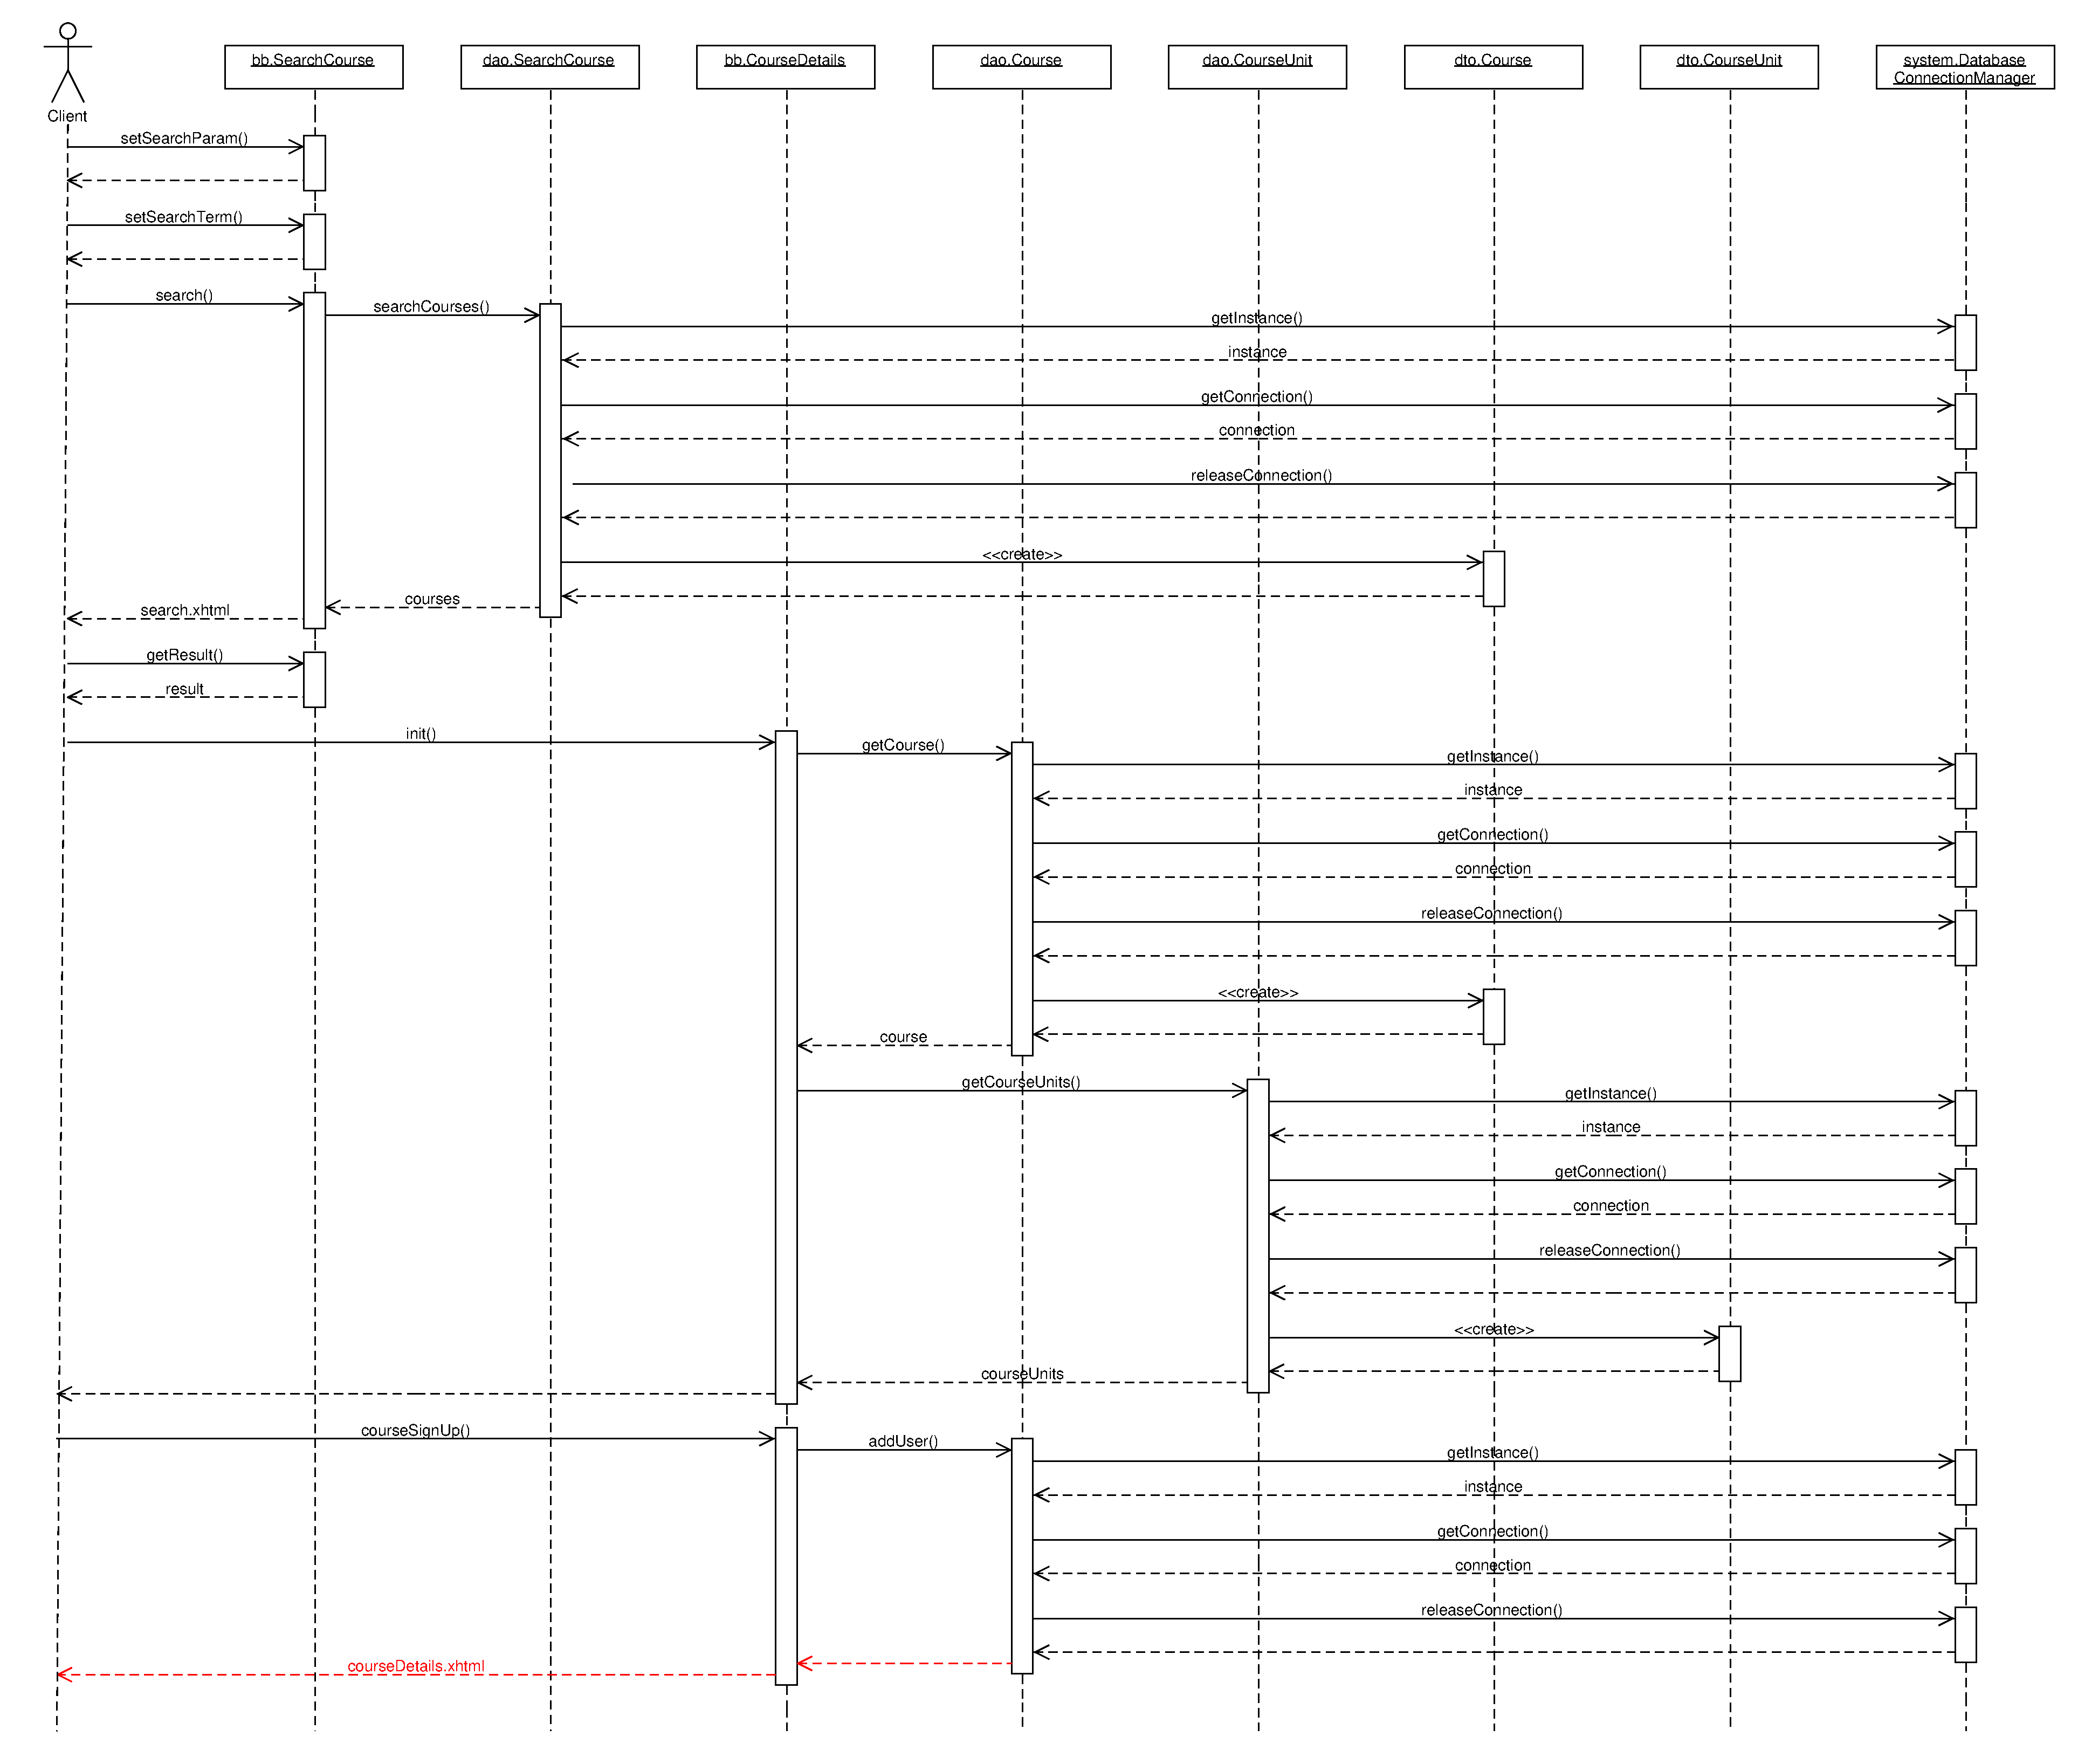
\includegraphics[scale=0.26]{./Grafiken/Sequenzdiagramm-Kursanmeldung.pdf}

\section{Konto aufladen}

\begin{tiny}
MB
\end{tiny}

Der eingeloggte Nutzer befindet sich auf der Seite buyCredits.xhtml zur Kontoaufladung. Dort werden alle relevanten Daten bezüglich der Kreditkarte angegeben, sowie der aufzuladene Betrag (siehe Kapitel 4.2.2 buyCredits.xhtml). Nach erfolgreicher Aufladung wird eine Bestätigung angezeigt.

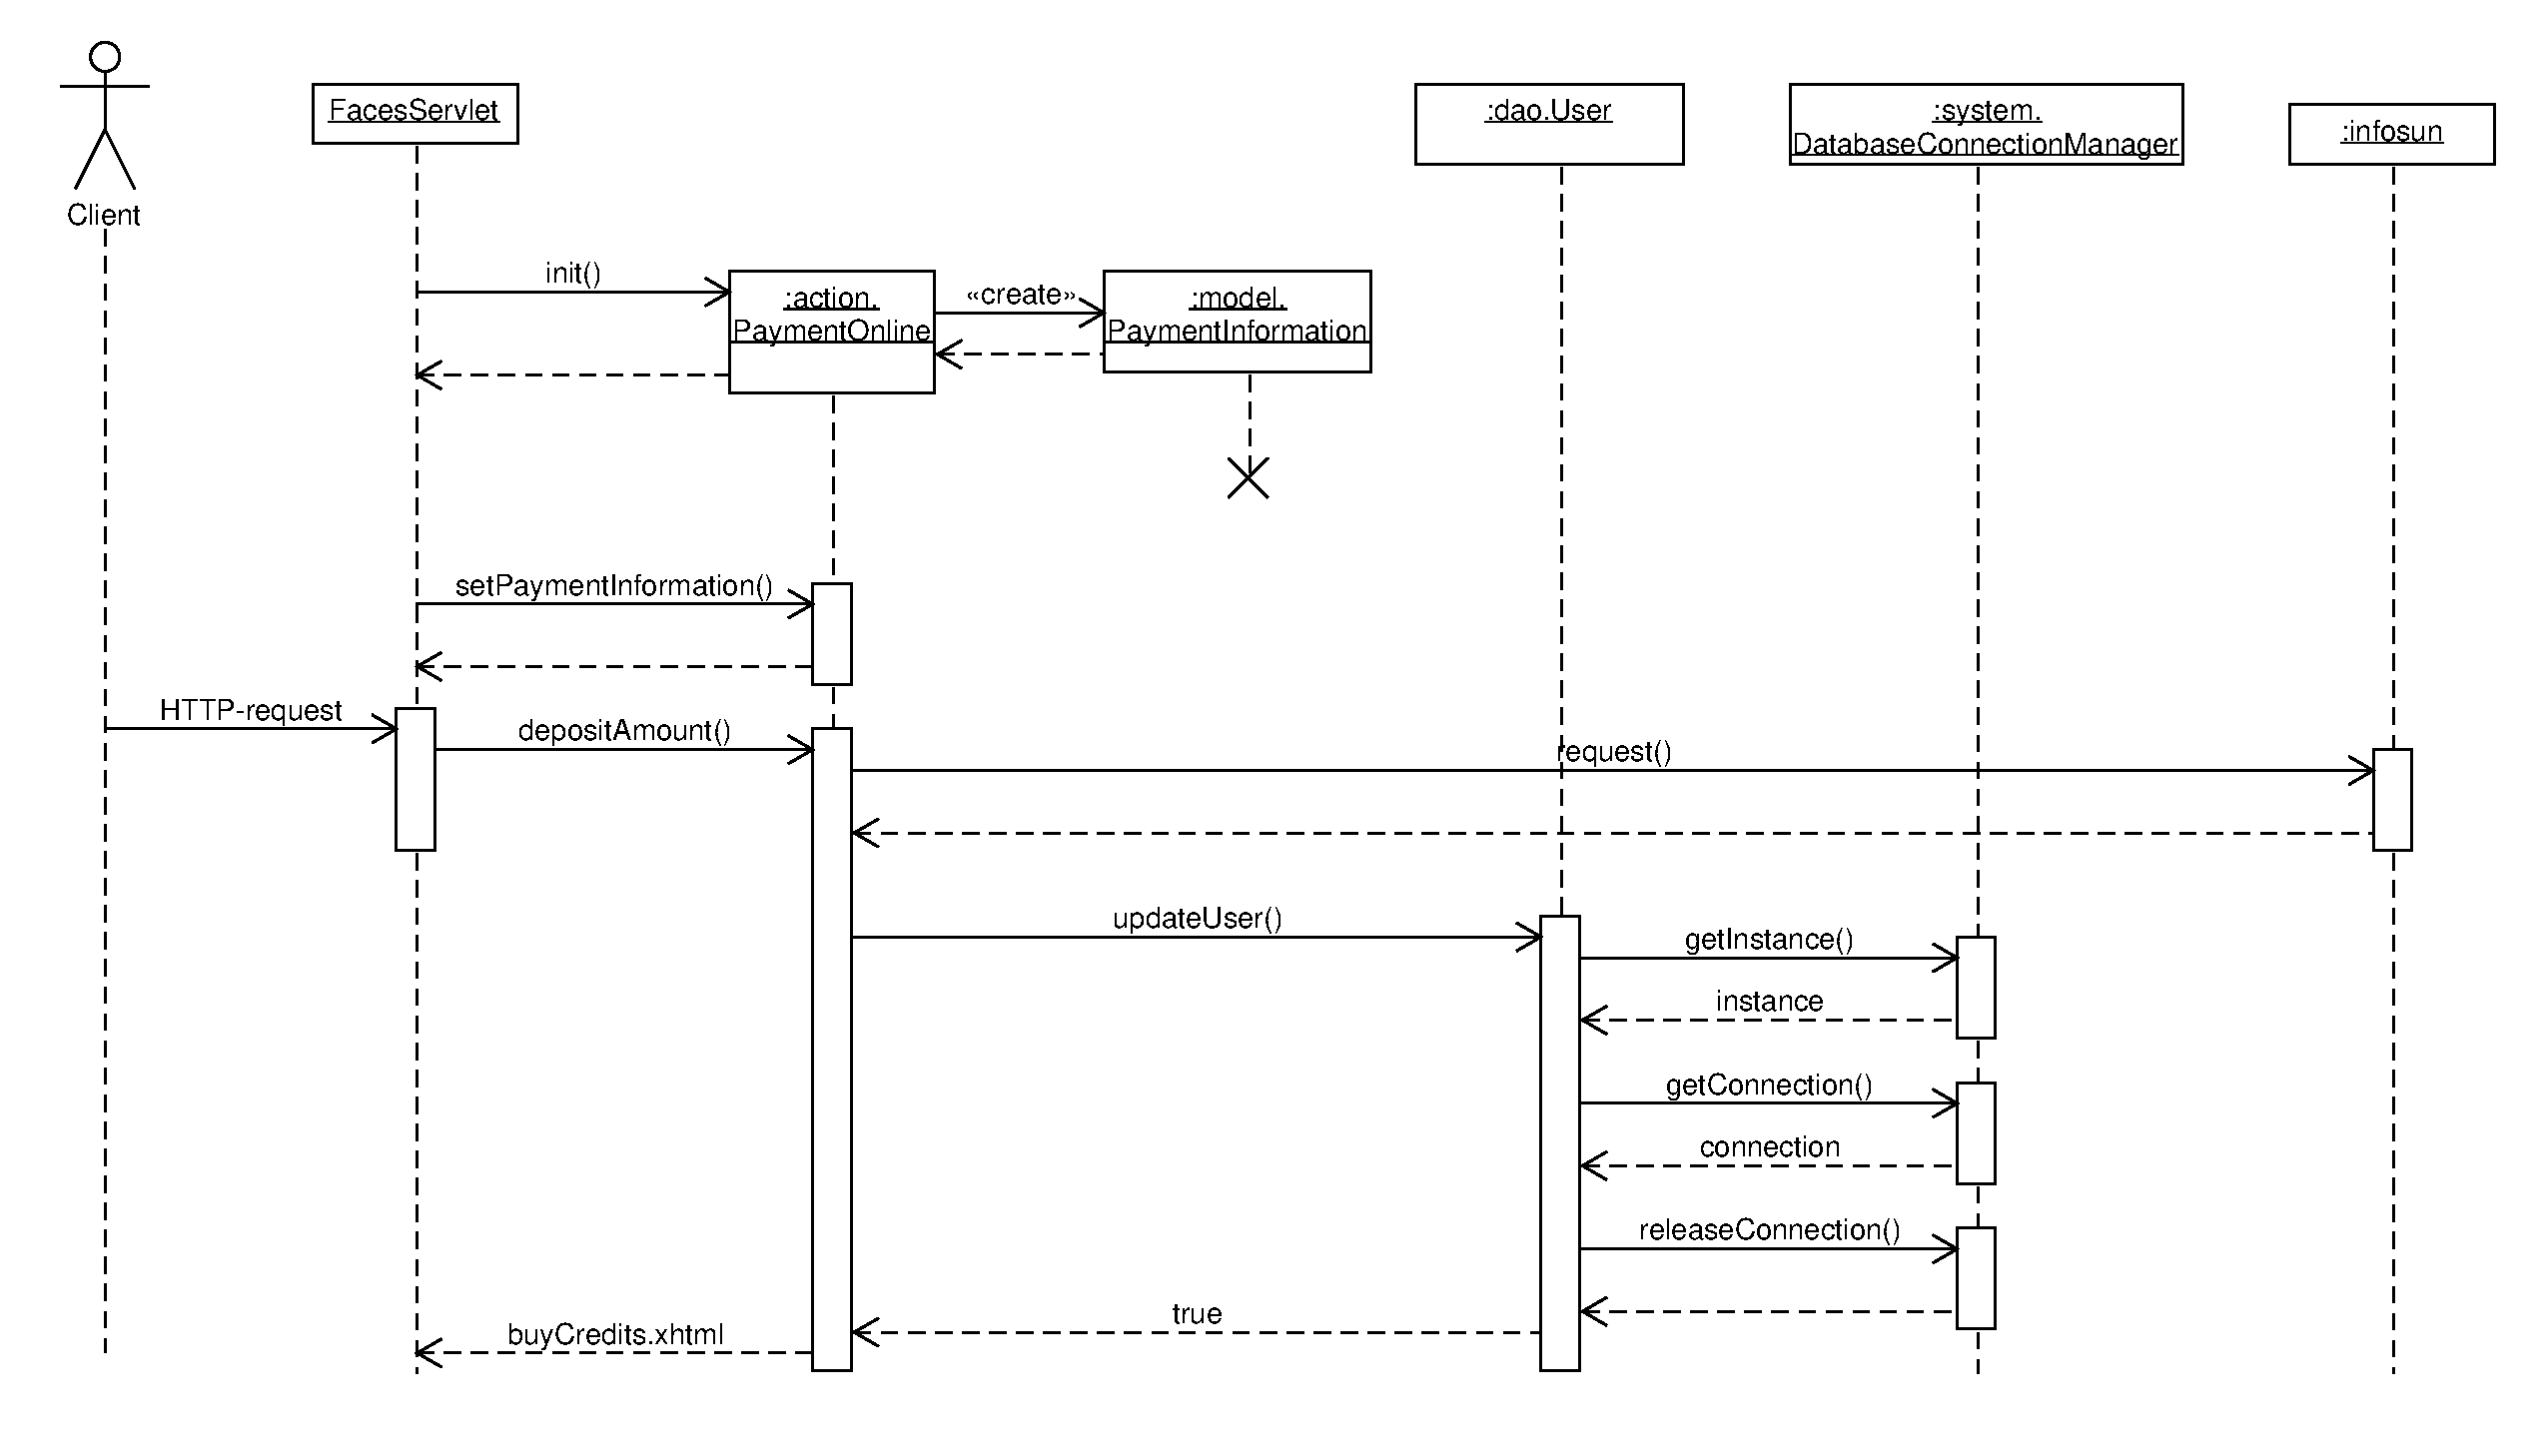
\includegraphics[scale=0.45]{./Grafiken/Sequenzdiagramm-KontoAufladung.pdf}